\documentclass[12pt]{article}

% =========================================================
% Language and font
% =========================================================
\usepackage{fontspec}
\setmainfont{Times New Roman}
\usepackage{polyglossia}
\setdefaultlanguage{serbian}
\newfontfamily\cyrillicfont{Times New Roman}
\newfontfamily\cyrillicfonttt{Times New Roman}

% =========================================================
% Page layout
% =========================================================
\usepackage[
    a4paper,
    top=2cm,
    bottom=2cm,
    left=2.5cm,
    right=2cm,
    heightrounded
]{geometry}

% =========================================================
% Text formatting
% =========================================================
\usepackage{setspace}
\setstretch{1.15}
\usepackage{indentfirst}
\setlength{\parindent}{1.25cm}
\setlength{\parskip}{0pt}

% =========================================================
% Mathematics
% =========================================================
\usepackage{amsmath, amssymb, amsthm}
\usepackage{mathrsfs}

% =========================================================
% Figures
% =========================================================
\usepackage{graphicx}
\usepackage{float}
\graphicspath{{figures/}}
\usepackage{caption}
\captionsetup{labelsep=space}
\usepackage{chngcntr}
\counterwithin{figure}{subsection}

% =========================================================
% Lists
% =========================================================
\usepackage[shortlabels]{enumitem}

% =========================================================
% URLs and hyperlinks
% =========================================================
\usepackage{xurl}
\usepackage{hyperref}
\hypersetup{
    colorlinks=true,
    linkcolor=black,
    urlcolor=blue,
    breaklinks=true
}

% =========================================================
% Other
% =========================================================
\usepackage{comment}


\title{Мастер рад}
\author{Лазар Попадић}
\date{Септембар 2026}
%\maketitle

\begin{document}
\tableofcontents
\newpage

\section{Увод}

\newpage
\section{Визуелна одометрија}

Шта је ВО? Шта све утиче на успешност ВО:
\begin{itemize}
    \item осветљеност,
    \item статична сцена,
    \item текстура и
    \item довољно преклапање узастопних слика.
\end{itemize}

Процена дубине у стерео. Дегенерација стерео у монокуларну. Процена дубине у монокуларној. Проблеми са неодређеношћу апсолутне скале. Подела метода ВО.

\subsection{SVO}
\subsection{ORB-SLAM3}
\subsection{TSformer-VO}
\subsection{Окружење}
С обзиром да су у овом раду коришћени алати и алгоритми који су развијени независно једни од других, јавила се потреба да се користе изолована развојна окружења. Коришћени су различити нивои изолације, у зависности од захтева појединачних алата. У наставку су наведена три алата која су коришћена за изолацију окружења:
\begin{itemize}
    \item \textit{Podman} контејнери,
    \item \textit{Conda} и
    \item \textit{Python venv}.
\end{itemize}
Контејнери представљају потпуну изолацију са комплетним оперативним системом и системским библиотекама. Окружење које је изоловано у контејнеру је независно од \textit{host} оперативног система. \textit{Conda} представља средњи ниво изолације и омогућава потпуну изолацију \textit{python} окружења од системског. \textit{Python venv} користи системски \textit{python} интерпретер и омогућава само одвајање инсталираних \textit{python} пакета. Избор алата који се користи за изолацију датог окружења зависи од системских зависности. Уколико је потребан одређен оперативни систем, користи се контејнер. Уколико је потребна другачија верзија \textit{python} интерпретера са свим осталим пакетима, користи се \textit{conda}. Уколико су потребне одређене верзије појединачних \textit{python} пакета, без потребе за мењањем интерпретера, користи се \textit{python venv}.

TODO: napisi sve ovo lepo





Verzije ROS-a direktno diktiraju verziju Ubuntu operativnog sistema; na primer, ROS1 Noetic je kompatibilan samo sa Ubuntu 20.04, što znači da algoritmi koji zavise od ROS1 nemaju izbora u pogledu operativnog sistema.
Jedan deo eksperimentalnog toka zahteva ROS1, C++ biblioteke, OpenCV i standardne ROS komponente (što nalaže Ubuntu 20.04), dok drugi deo zahteva modernije Python okruženje sa novijim bibliotekama, koje su pogodnije za Ubuntu 24.04.
Ako bi se sve instaliralo u jedno okruženje, javili bi se konflikti između verzija paketa, Python interpretatora, biblioteka i ROS zavisnosti.
Zbog toga je bilo neophodno koristiti separisana okruženja za različite funkcionalne potrebe.
2) Zašto su korišćeni kontejneri
Kontejneri omogućavaju izolaciju softverskih zavisnosti bez menjanja celokupnog razvojnog sistema na hostovskoj mašini.
Svaki kontejner je bio namenjen drugoj fazi istraživanja: jedan za ROS1 testiranje algoritama, drugi za Python analizu i evaluaciju rezultata.
3) ROS1, SVO i ORB-SLAM3 zavisnosti
SVO i ORB-SLAM3 algoritmi zavise od ROS1 kompatibilne implementacije i standardnog ROS ekosistema.
Testiranje ovih algoritama mora da bude realizovano u okruženju koje odgovara njihovim originalnim zahtevima.
4) Zašto je korišćen Conda
Conda je korišćena za projekte čije su zavisnosti specifične i teško kompatibilne sa sistemskim Python-om.
U ovom radu je Conda korišćena za rad sa TSformer-VO i za evaluacione alate vezane za KITTI odometriju.
5) Zašto je korišćen Python venv
Python venv je korišćen za lokalno, lagano i ograničeno Python okruženje, bez potrebe za potpuno novim instalacionim sistemom.
On je koristan kada je potrebno da se određena Python aplikacija ili alat pokrene sa minimalnim skupom biblioteka, a da se ne menja globalni sistemski Python.
U ovom radu je venv korišćen za alate vezane za obradu bag fajlova i druge Python skripte za konverziju i analizu podataka.
Venv je bio pogodniji od Conda za manje, fokusirane i lokalne Python zadatke.
6) Šta je korišćeno za šta
ROS1/Ubuntu 20.04 okruženje: testiranje i validacija algoritama SVO i ORB-SLAM3, rad sa ROS paketima, ROS temama i bag fajlovima, pokretanje algoritama u okruženju koje odgovara njihovoj originalnoj implementaciji.
Modernije okruženje / Ubuntu 24.04: razvojni i analitički deo rada, obrada datoteka i dataset-a, evaluacija rezultata, rad sa novijim Python i OpenCV paketima.
Conda: TSformer-VO eksperimenti, KITTI odometrijska evaluacija, okruženja sa specifičnim Python i dependency zahtevima.
Python venv: lokalni Python alati za konverziju i obradu bag podataka, jednostavna i fokusirana Python okruženja.



\newpage

\section{Прикупљање података}

\subsection{Робот}
Положај камере убаци овде, да не буду два наслова за камеру.
\begin{figure}[H]
    \centering
    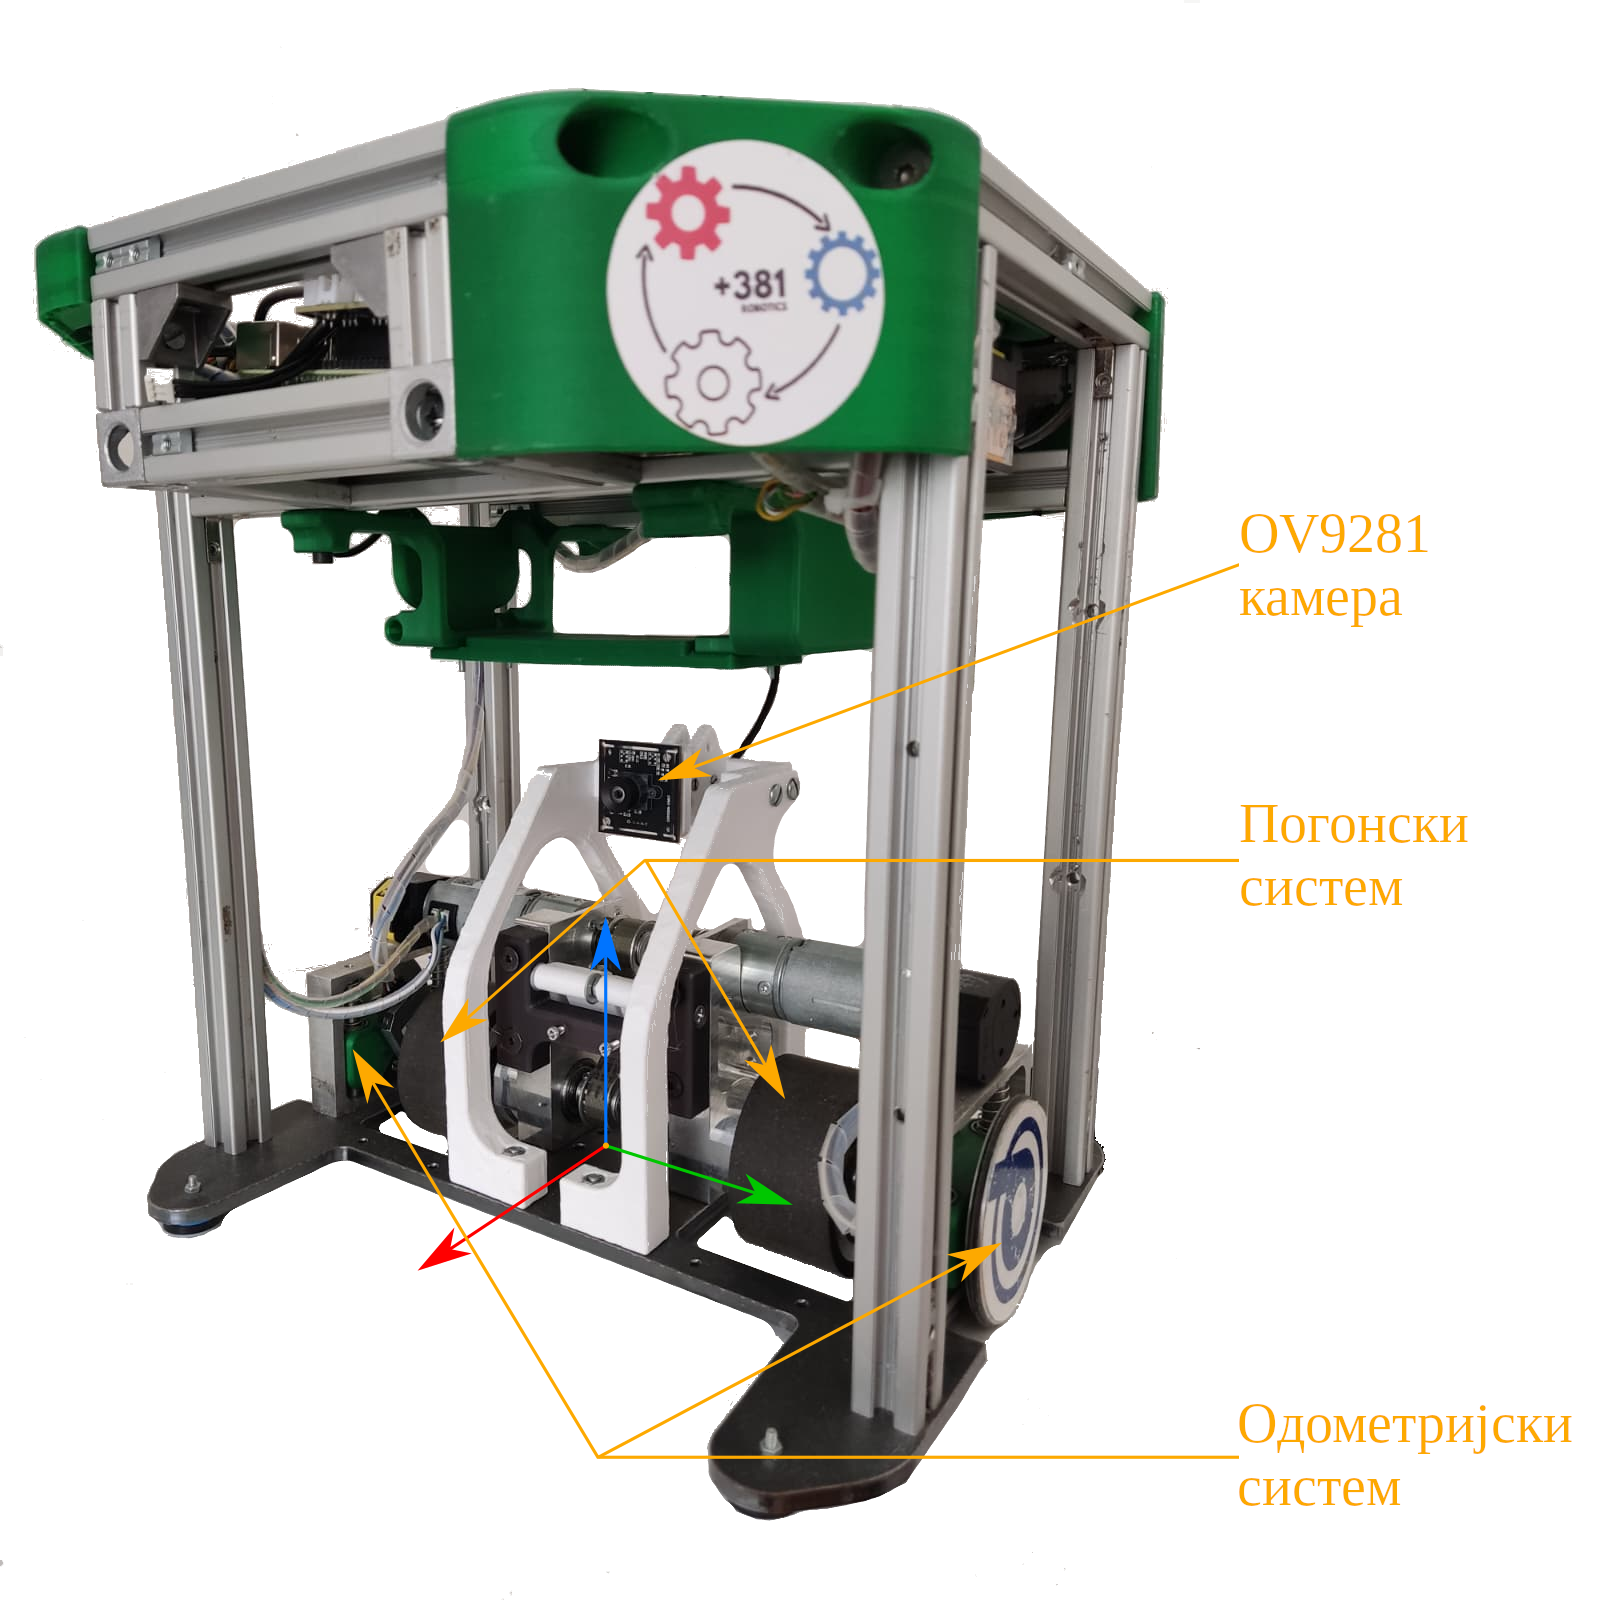
\includegraphics[width=12cm]{figures/robot.png}
    \caption{Робот тима +381 \textit{Robotics}}
    \label{fig:робот}
\end{figure}
\subsubsection{Диференцијални погон}
Два независно актуисана саосна точка. Два степена слободе. Нехолономно ограничење. Три типа кретања. 

\subsubsection{Одометријски систем}
Инкрементални енкодери на пасивним точковима. Одвојен од погонског због проклизавања погонских точкова.
Објасни кинематски модел са слике.
\begin{figure}[H]
    \centering
    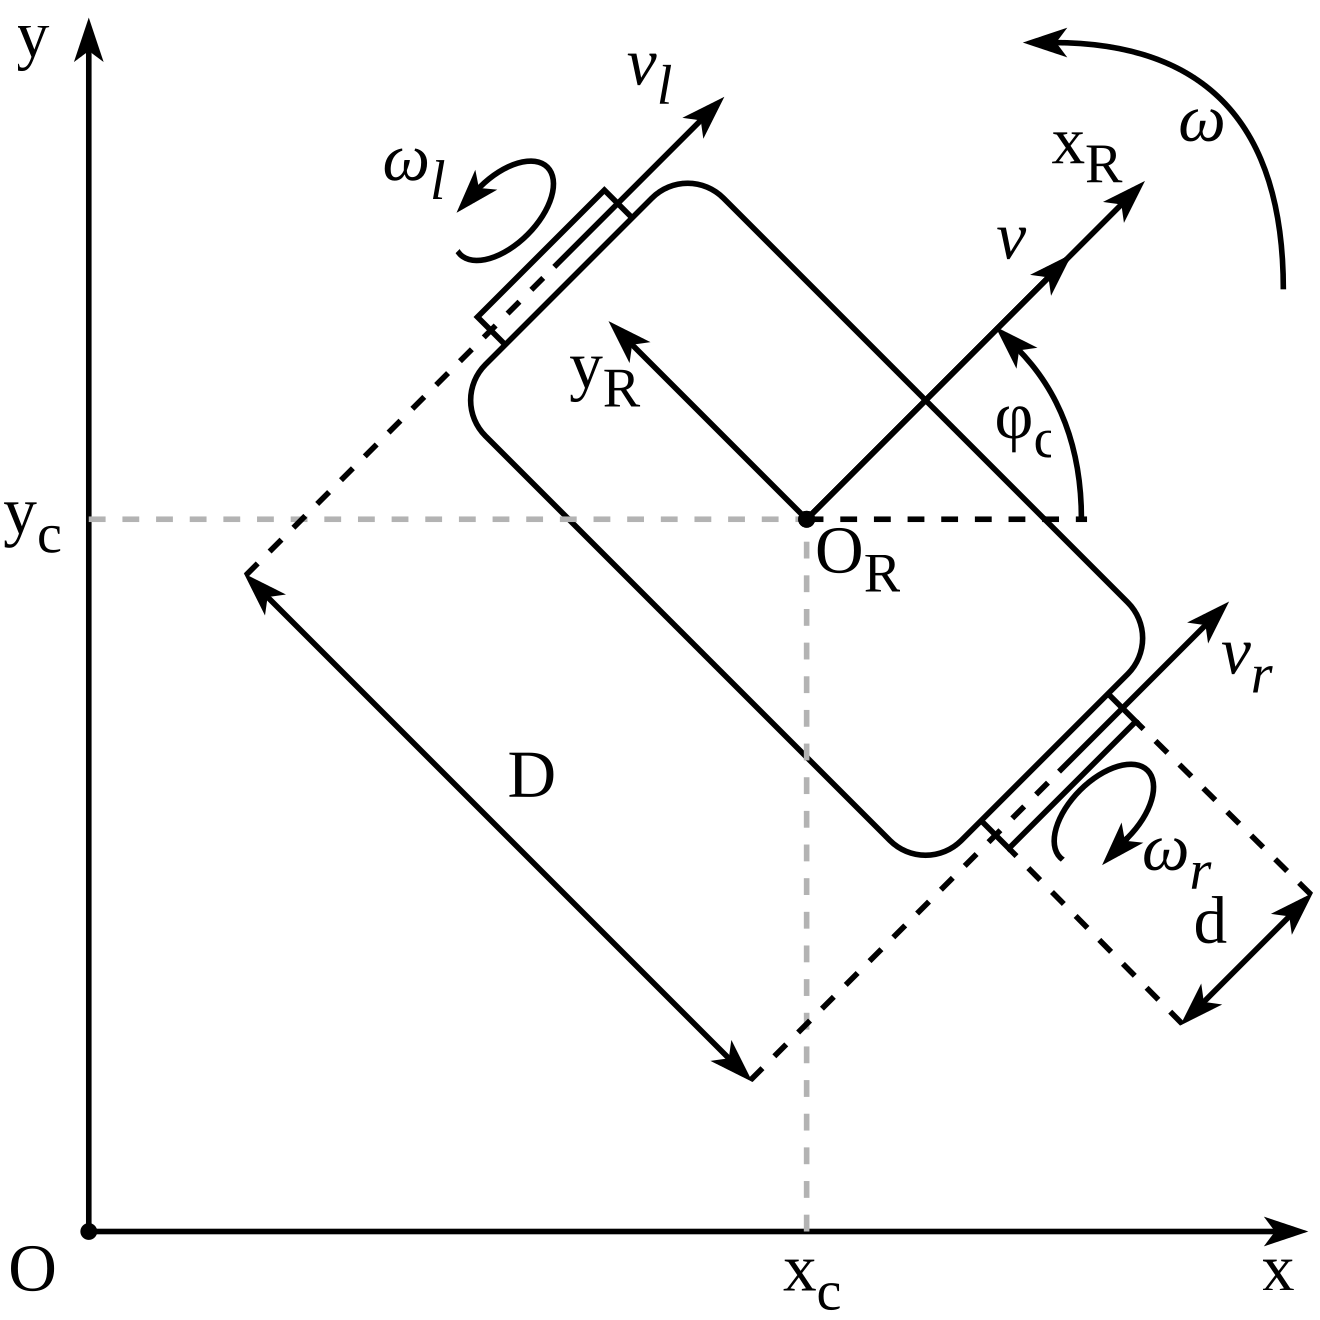
\includegraphics[width=12cm]{figures/diff_kinematic_model.png}
    \caption{Кинематски модел диференцијалног робота}
    \label{fig:кинематски_модел}
\end{figure}
TODO: sredi malo ovu recenicu:
Једначине кинематског модела:
\begin{equation}
    v_r = \omega_r \cdot \dfrac{d}{2}
\end{equation}
\begin{equation}
    v_l = \omega_l \cdot \dfrac{d}{2}
\end{equation}
\begin{equation}
    v = \dfrac{v_r + v_l}{2}
\end{equation}
\begin{equation}
    \omega = \dfrac{v_r - v_l}{D}
\end{equation}
\begin{equation}
    x_c^{k+1} = x_c^k + v \cdot \cos(\varphi_c^k + \dfrac{\omega \cdot \Delta t}{2}) \cdot \Delta t
\end{equation}
\begin{equation}
    y_c^{k+1} = y_c^k + v \cdot \sin(\varphi_c^k + \dfrac{\omega \cdot \Delta t}{2}) \cdot \Delta t
\end{equation}
\begin{equation}
    \varphi_c^{k+1} = \varphi_c^k + \omega \cdot \Delta t
\end{equation}

Значења ознака су:
\begin{itemize}
    \item $O$, $x$, $y$ - референтни координатни систем
    \item $O_R$, $x_R$, $y_R$ - локални координатни систем робота
    \item $x_c$, $y_c$, $\varphi_c$ - положај и оријентација робота у референтном систему
    \item $v$ - линеарна брзина базе робота
    \item $\omega$ - угаона брзина базе робота
    \item $\omega_r$, $\omega_l$ - угаона брзина десног и левог одометријског точка
    \item $v_r$, $v_l$ - линеарна брзина десног и левог одометријског точка
    \item $D$ - растојање између одометријских точкова
    \item $d$ - пречник одометријских точкова
    \item $\Delta t$ - временски интервал између два одбирка
    \item $k$, $k+1$ - тренутни и наредни одбирак
\end{itemize}

\subsection{\textit{Rosbag}}
Основно за \textit{ROS}. Снимани топици...

\newpage

\subsection{Камера}
\subsubsection{Калибрација}

\subsection{Секвенце}
Физичко окружење не мора у свој поднаслов.
Опис секвенци и брзина.
Разлог за избор секвенци.
\subsubsection{Процена референтних путања}
Зашто не може само одом са точкова. Прорачунате грешке у секвенцама.
"Стековање" у зид. Апроксимације које су коришћене при процени референтних путања.

\newpage


\section{Резултати и дискусија}
Текст.
\newpage

\section{Закључак}
Текст.
\newpage

\section{Прилог}
\subsection{Прилог А}
\begin{figure}[H]
    \centering
    \includegraphics[width=17.5cm]{figures/+381Logo.png}
    \caption{Функција за директну кинематику у \textit{MATLAB}-у}
    \label{fig:direktna_kinematika_matlab}
\end{figure}
\newpage

\subsection{Први поднаслов}
Нешто из литературе [1]. Пример је приказан на слици 2.1.1.

\begin{figure}[H]
    \centering
    \includegraphics[width=12cm]{figures/abb_irb_140.jpg}
    \caption{Серијски манипулатор антропоморфне конфигурације \textit{ABB IRB} 140 [2]}
    \label{fig:серијски_манипулатор}
\end{figure}

На слици 2.1.2 је приказан други пример.

\begin{figure}[H]
    \centering
    \includegraphics[width=12cm]{figures/abb_irb_360.jpg}
    \caption{Паралелни манипулатор делта конфигурације \textit{ABB IRB} 360 [2]}
    \label{fig:паралелни_манипулатор}
\end{figure}

Пример списка:
\begin{itemize}
    \item већа крутост кинематског ланца
    \item мања маса манипулатора
    \item већа носивост
    \item боља прецизност, као последица мањих деформација
\end{itemize}

\subsubsection{Први подподнаслов}
Сингуларне конфигурације су одређени положаји крајњег ефектора, за које паралелни роботи губе своју инхерентну бесконачну крутост и у којима крајњи ефектор има неконтролисане степене слободе [1]. Типови кинематских сингуларитета су:
\begin{itemize}
    \item Тип 1. За ненулти вектор улазних брзина, крајњи ефектор се не креће.
    \item Тип 2. Крајњи ефектор се креће при нултом вектору улазних брзина.
    \item Тип 3. Комбинација сингуларитета типа 1 и 2. Могуће је кретање крајњег ефектора без кретања улазних сегмената и обрнуто, могуће је кретање улазних сегмената без кретања крајњег ефектора.
\end{itemize}

\subsubsection{Други подподнаслов}
Текст.
Примери једначина: $\vec{M}_{in} - I\vec{\alpha} = 0$, $\vec F=Q(\vec v \times \vec B)$, $e_a=-N\dfrac{\partial\phi }{\partial t}$.

\subsubsection{Трећи подподнаслов}

\subsection{Други поднаслов}
Текст.
У прилогу А је MATLAB функција која служи за израчунавање директне кинематике.

\subsection{\textit{Subsection name in English}}
Текст.

\section{Литература}
\begin{enumerate}[start=1,label={[\arabic*]}]
\item J. P. Merlet, Parallel Robots, 2nd ed. Springer 2006
\item \url{https://new.abb.com/en}
\item \url{http://mehanizacija.ftn.uns.ac.rs/wp-content/uploads/2021/02/7.-DINAMICKA-ANALIZA-mehatronika-2019.pdf}, Механика машина, др М. Чавић, редовни професор, МСц Д. Чавић, асистент
\item D. K. Sen, A. Yildiz, O. Kopmaz, "Optimal Design of a Five-Bar Planar Manipulator and Its
Controller by Using Different Algorithms for Minimum
Shaking Forces and Moments for the Largest Trajectory in a
Usable Workspace", MDPI, Machines 2022, 10, 971.
\item \url{https://www.keep.ftn.uns.ac.rs/regulisani-elektromotorni-pogoni/specifikacija/specifikacija-predmeta/}, Регулисани електромоторни погони, др Д. Марчетић, редовни професор, МСц В. Поповић, доцент
\item др Д. Јеркан, Б. Вујков, Збирка задатака из електричних машина за студијски програм мехатроника, Нови Сад, ФТН 2020
\item \url{http://www.automatika.ftn.uns.ac.rs/images/predmeti/Sistemi%20automatskog%20upravljanja%20-%20mehatronika/Predavanja/10_Regulacija.pdf}, Системи аутоматског управљања,
др А. Ристић, редовни професор, др В. Бугарски, доцент
\item F. Marini, B. Walczak, "Particle swarm optimization (PSO). A tutorial", Elsevier 2015
\item Ж. Кановић, З. Јеличић, М. Рапаић, Еволутивни оптимизациони алгоритми у инжењерској пракси, Нови Сад, ФТН 2017
\end{enumerate}

\end{document}
